% ============================================================================
% The True Lethality Engine — final project report
% Statistical Machine Learning, Sapienza Università di Roma
%
% Build:  pdflatex report.tex  (twice, for references)   or:  make report
% Figures are pulled live from ../figures/ — recompile after `make retrain`
% or `make battlecast` and the report stays in sync with the artifacts.
% ============================================================================
\documentclass[10pt,twocolumn]{article}

\usepackage[T1]{fontenc}
\usepackage[utf8]{inputenc}
\usepackage[a4paper,margin=2cm,columnsep=0.8cm]{geometry}
\usepackage{lmodern}
\usepackage{amsmath,amssymb}
\usepackage{booktabs}
\usepackage{graphicx}
\usepackage{xcolor}
\usepackage[hidelinks]{hyperref}
\usepackage{microtype}
\graphicspath{{../figures/}}

\definecolor{sapienzaRed}{RGB}{130,36,51}
\usepackage{titlesec}
\titleformat{\section}{\large\bfseries\color{sapienzaRed}}{\thesection}{0.6em}{}
\titleformat{\subsection}{\normalsize\bfseries\color{sapienzaRed}}{\thesubsection}{0.6em}{}
\setlength{\parskip}{2pt}

\newcommand{\code}[1]{\texttt{\small #1}}

\title{\color{sapienzaRed}\textbf{The True Lethality Engine}\\
\large\color{black} Predicting the real danger of D\&D 5e combat from 34{,}907 recorded encounters}
% TODO: add surnames / matricole before submission
\author{Daniele \,\textperiodcentered\, Francesca \,\textperiodcentered\, Stefano \,\textperiodcentered\, Antonietta\\[2pt]
\small Statistical Machine Learning --- Final Project, Sapienza Università di Roma, A.Y.~2025/2026\\
\small \url{https://dnd-appraising.streamlit.app} \quad
\url{https://github.com/danpinocontrollino/project-dnd}}
\date{}

\begin{document}
\maketitle

\begin{abstract}
\noindent
Dungeons \& Dragons 5e rates every monster with a \emph{Challenge Rating} (CR), a
designer-assigned difficulty score that has never been validated against actual play.
We validate it --- and replace it. From 153{,}829 turn snapshots of real online play
(the FIREBALL corpus) we build 34{,}907 encounter-level observations across 1{,}462
campaigns, parse offensive statistics directly out of monster statblock text, and train
a calibrated, monotonicity-constrained XGBoost model of $\eta(x)=P(\text{party wins}\mid x)$.
Inverting $\eta$ by binary search yields the \emph{True Lethality Level}: the party level
at which a balanced party of four reaches a target win rate. Validation is grouped by
campaign --- the true unit of leakage --- giving an honest held-out ROC--AUC of
0.657 (95\% bootstrap CI $[0.638, 0.674]$) and Brier score 0.139 $[0.134, 0.145]$ at an
83\% base rate. Because observational play is contaminated by ``DM mercy'' (fights the
damage math deems hopeless were still recorded as wins 84.5\% of the time), the engine
adds three explicit domain guards; the survival guard's constants are calibrated
externally against 490{,}640 simulated fight-to-the-death battles. Along the way, a ridge
logistic model \emph{wins} on observational AUC (0.655 vs.\ 0.614) yet is rejected: its
confounded coefficients make it unusable for the interventional questions the
application asks. The result is a live encounter appraiser that measures the rulebook
against the data --- with the rulebook's own math implemented honestly.
\end{abstract}

\section{Introduction}
In D\&D 5e a party of 3--6 heroes (levels 1--20) fights monsters run by a Dungeon
Master (DM). The official difficulty currency is the Challenge Rating: a CR-$k$
monster should challenge four level-$k$ heroes, and the \emph{Dungeon Master's
Guide} (DMG, p.~82) grades encounters by comparing multiplier-adjusted monster XP
against per-level thresholds~\cite{dmg}. CR is a design intention: it compresses
offense, defense, traits and action economy into one printed number, and its known
failure modes (high-CR solos folding to action economy, deadly low-CR swarms, trait
synergies) had never been quantified against play. We ask a precisely defined
question instead:

\smallskip
\noindent\emph{What is the calibrated probability $\eta(x)$ that a given party wins a
given encounter $x$ --- and at which party level $L$ does a balanced party of four
reach a chosen target win rate (default 65\%)?}
\smallskip

$L$, found by binary search on $\eta$ over levels $[1,20]$ (18 iterations, quarter-level
rounding), is the \textbf{True Lethality Level}. Boundary cases get explicit verdicts
rather than fabricated precision: \emph{trivial} ($\eta\ge$ target at level~1) and
\emph{beyond deadly} ($\eta<$ target at level~20, reported with its ceiling).

\textbf{Contributions.} (i)~an encounter-level dataset distilled from real play, with
offensive statistics parsed from statblock text; (ii)~a calibrated, shape-constrained
model with campaign-grouped validation and bootstrap uncertainty; (iii)~a diagnosis of
estimand mismatch in observational game data (``DM mercy'') and a three-guard
architecture, one guard calibrated by external simulation; (iv)~a course-toolbox
benchmark (penalized logistic, random-feature kernel machine, MMD test, Gaussian
process) with a decision-theoretic model-selection lesson; (v)~a deployed application
that compares the model against the DMG's own procedure, implemented faithfully.

\section{Data}
\subsection{From chat logs to encounters}
FIREBALL~\cite{fireball} collects real games played on Discord through the Avrae bot.
Our ETL (\code{parse\_fireball.py}) processes 1{,}471 JSONL logs (153{,}829 turn
snapshots; 134{,}475 valid turns), infers outcomes from terminal HP states, drops
85{,}778 unresolved fights and 9{,}215 encounters with no bestiary match, and emits
\textbf{34{,}907 resolved encounters} across \textbf{1{,}462 campaigns}. The party
win base rate is \textbf{83.0\%} --- a number that shapes everything downstream.
Each row has 29 raw columns: party level/size and four role flags (healer, tank,
arcane, martial DPS, mapped from character classes), roster aggregates
(count-weighted means for continuous statistics, maxima for binary traits and apex
threats, pooled sums for the damage race), ten monster trait flags, XP totals, and
the outcome. Party levels are clipped to $[1,20]$ and rosters to 30 (mass-summon
logs reach 241 actors).

\subsection{The Attack Potency problem}
Monster manuals list HP and AC but no machine-readable offense. We parse it from the
SRD statblock text itself: attack bonuses (\code{+9 to hit}), printed average damage
(\code{12 (2d6+5)}), multiattack routines (``makes \emph{three} attacks''), save DCs, and
spell lists priced by a 30-spell PHB damage table. Per-action segmentation separates
\emph{sustained} DPR (weapon routine) from \emph{burst} (the single scariest action):
the Lich yields DPR 45 and burst 100 (\emph{Power Word Kill}). Coverage: 321/762
monsters from real statblocks, the remainder imputed from the DMG's design table by
CR; parsed DPR is clamped to $[0.25\times,3\times]$ of the design band. Regression
tests caught two real bugs: versatile weapons double-counted (24 monsters) and dragon
breath leaking into multiattack math (Adult Red Dragon 72.6\,$\to$\,58; hand-computed
truth $\approx$45--48). Spot checks: Goblin 5 (true 5), Tarrasque 150 (true $\approx$148).

\subsection{Playing fair with the rulebook}
If we claim to beat the DMG we must implement it correctly. The application's
``by-the-book'' verdict runs the full p.~82 procedure --- total XP, the count
multiplier ladder with the p.~83 party-size adjustment, and an inverse XP lookup to an
equivalent single-monster CR --- so that $6\times$CR-1 monsters read as one CR-6
encounter, not ``CR~1''. The implementation passes nine regression tests including the
DMG's own worked example; reported discrepancies therefore measure the model against
the rulebook's best effort, not a strawman.

\section{Methods}
\subsection{Features: combat math as covariates}
Forty-five features in five families: raw party/roster aggregates (15); offensive
potency (5); power curves and ratios (6); trait$\times$composition interactions such
as \emph{magic resistance}$\times$\emph{arcane party} (6); and combat mathematics plus
the DMG budget (13) --- to-hit probabilities on both sides from the actual d20 rule,
rounds-to-kill in both directions with a log-ratio, nova pressure
(\code{burst\_vs\_pc\_hp}), and the multiplier-adjusted XP budget. All feature
engineering lives inside a serialized \code{sklearn} transformer, so training and
serving cannot drift.

\subsection{Model and calibration}
The production model is XGBoost~\cite{xgboost} (300 trees, depth 4, learning rate
0.149, subsample 0.68, column subsample 0.85, $\lambda$=0.105, $\alpha$=0.091,
$\gamma$=0.009; tuned by Optuna~\cite{optuna} against a grouped-CV objective, study
persisted) under \textbf{45 monotone constraints}: party level, size and role flags
positive; monster count, CR, HP, DPR, burst, attack bonus, save DC and every hostile
trait negative. Constraints double as the out-of-distribution guard: inputs are also
clipped to legal 5e bands before featurization. Probabilities are calibrated with
Platt scaling~\cite{platt} on \emph{campaign-grouped} folds. Isotonic calibration
was evaluated and rejected: its piecewise-constant map collapsed the level search
(one Lich $\equiv$ two Liches) while measuring marginally worse (Brier 0.1394 vs.\
0.1397).

\subsection{Validation protocol}
Encounters within a campaign share party, DM and house rules, so the campaign is the
unit of leakage. Everything is grouped by it: \code{StratifiedGroupKFold}
cross-validation, a grouped 80/20 holdout ($n_{\text{test}}{=}7{,}106$), and the
calibration folds themselves. Headline metrics carry 95\% percentile-bootstrap CIs
(2{,}000 resamples). A kernel two-sample test (unbiased MMD$^2$~\cite{mmd}, RBF with
median-heuristic bandwidth, permutation null) between train- and held-out-campaign
feature distributions gives MMD$^2{=}3.1\times10^{-4}$, $p{=}0.12$: no detectable
covariate shift, so the grouped-CV/holdout gap reflects campaign-level outcome
variance rather than distribution drift.

\section{Where the data lies: guards and simulation}
\subsection{DM mercy}
An early model rated \emph{nineteen} CR-21 Liches as beatable by a level-8 party.
The cause is in the world, not the code: in fights the deterministic damage race
declares hopeless (party deleted in $\le$1 round), the logs still record a party win
\textbf{84.5\%} of the time (659 rows) --- fudged rolls, retreats recorded as wins,
reinforcements. The logs answer ``what happens at real tables''; the application asks
``what if you fought \emph{to the death}''. That is an estimand mismatch no amount of
identically-collected data can repair.

\subsection{Three guards}
(1)~\emph{Shape priors and clipping} (above). (2)~\emph{Roster dominance}: count-weighted
averages dilute --- a Lich with 2 ogres and 6 goblins has mean CR 2.94 versus the
Lich's 21, and the raw model rated the larger fight easier (level 3.25 vs.\ 5.0); the
engine therefore also scores every homogeneous sub-roster and returns the
\emph{minimum} win probability, enforcing the axiom that adding monsters can never
help the party. (3)~A \emph{survival physics cap}
$P(\text{win}) \le \sigma(a\cdot\mathrm{TTK}+b)$, where TTK is the deterministic
rounds-to-kill-the-party computed from the same feature mathematics the model trains
on --- smooth, monotone in level and decreasing in roster damage, so the binary search
and dominance guarantees survive.

\subsection{Calibrating the guard by simulation}
Hand-tuned constants are a confession, so we replaced them. We vendored the public
Monte Carlo engine of Battlecast (a 5e combat simulator resolving initiative,
movement, spell slots and conditions with scripted play and \emph{no} mercy) and ran
a designed grid of \textbf{304 cells $\times$ 2{,}000 trials = 490{,}640 battles}
(party fixed to Fighter/Cleric/Wizard/Rogue): a 180-cell guard grid (boss CR
$\{2,5,10,15,21\}\times$ count $\{1..19\}\times$ level $\{1..20\}$), a 100-cell
``mercy'' grid (25 SRD monsters $\times$ 4 levels), and a 24-cell OOD grid (HP
$\times\{1,5,20\}$, AC $+\{0,8\}$ clones). A binomially-weighted logistic fit of
simulated $P(\text{win})$ on TTK gives
\[
\sigma(1.63\,\mathrm{TTK} - 3.98) \quad \text{replacing} \quad \sigma(2.197\,\mathrm{TTK}-4.394),
\]
i.e.\ caps of 9\%/33\%/71\% at 1/2/3 rounds of survival (the hand guess was too
generous in the 2--3-round zone), inert above ${\approx}3.7$ rounds where training
data is trustworthy (Fig.~\ref{fig:guard}). The deployed Lich ladder becomes
$1\to3.25$, $2\to6.75$, $4\to12.75$, $8{+}\to$ \emph{beyond deadly} (19 Liches:
$P(\text{win})$ at level 20 $=9.1\%$).

Pairing both lenses on the mercy grid quantifies the bias (Fig.~\ref{fig:mercy}):
correlation 0.845, with a \emph{crossover} --- the model sits ${\approx}{+}0.32$
above the simulator on hard fights (mercy inflation; few cells, directional) and
${\approx}{-}0.14$ below on easy ones (the 83\% ceiling from retreats and noisy
labels). On the OOD grid the extremes agree exactly (HP$\times$20 clones win
0.000--0.003 of deathmatches) while fine mid-range ordering is only moderate
(Spearman $\rho{=}0.54$). Caveats: the simulator implements 2024-SRD rules versus
2014-era logs, and scripted optimal play makes deathmatch rates an upper bound.

\begin{figure}[t]
  \centering
  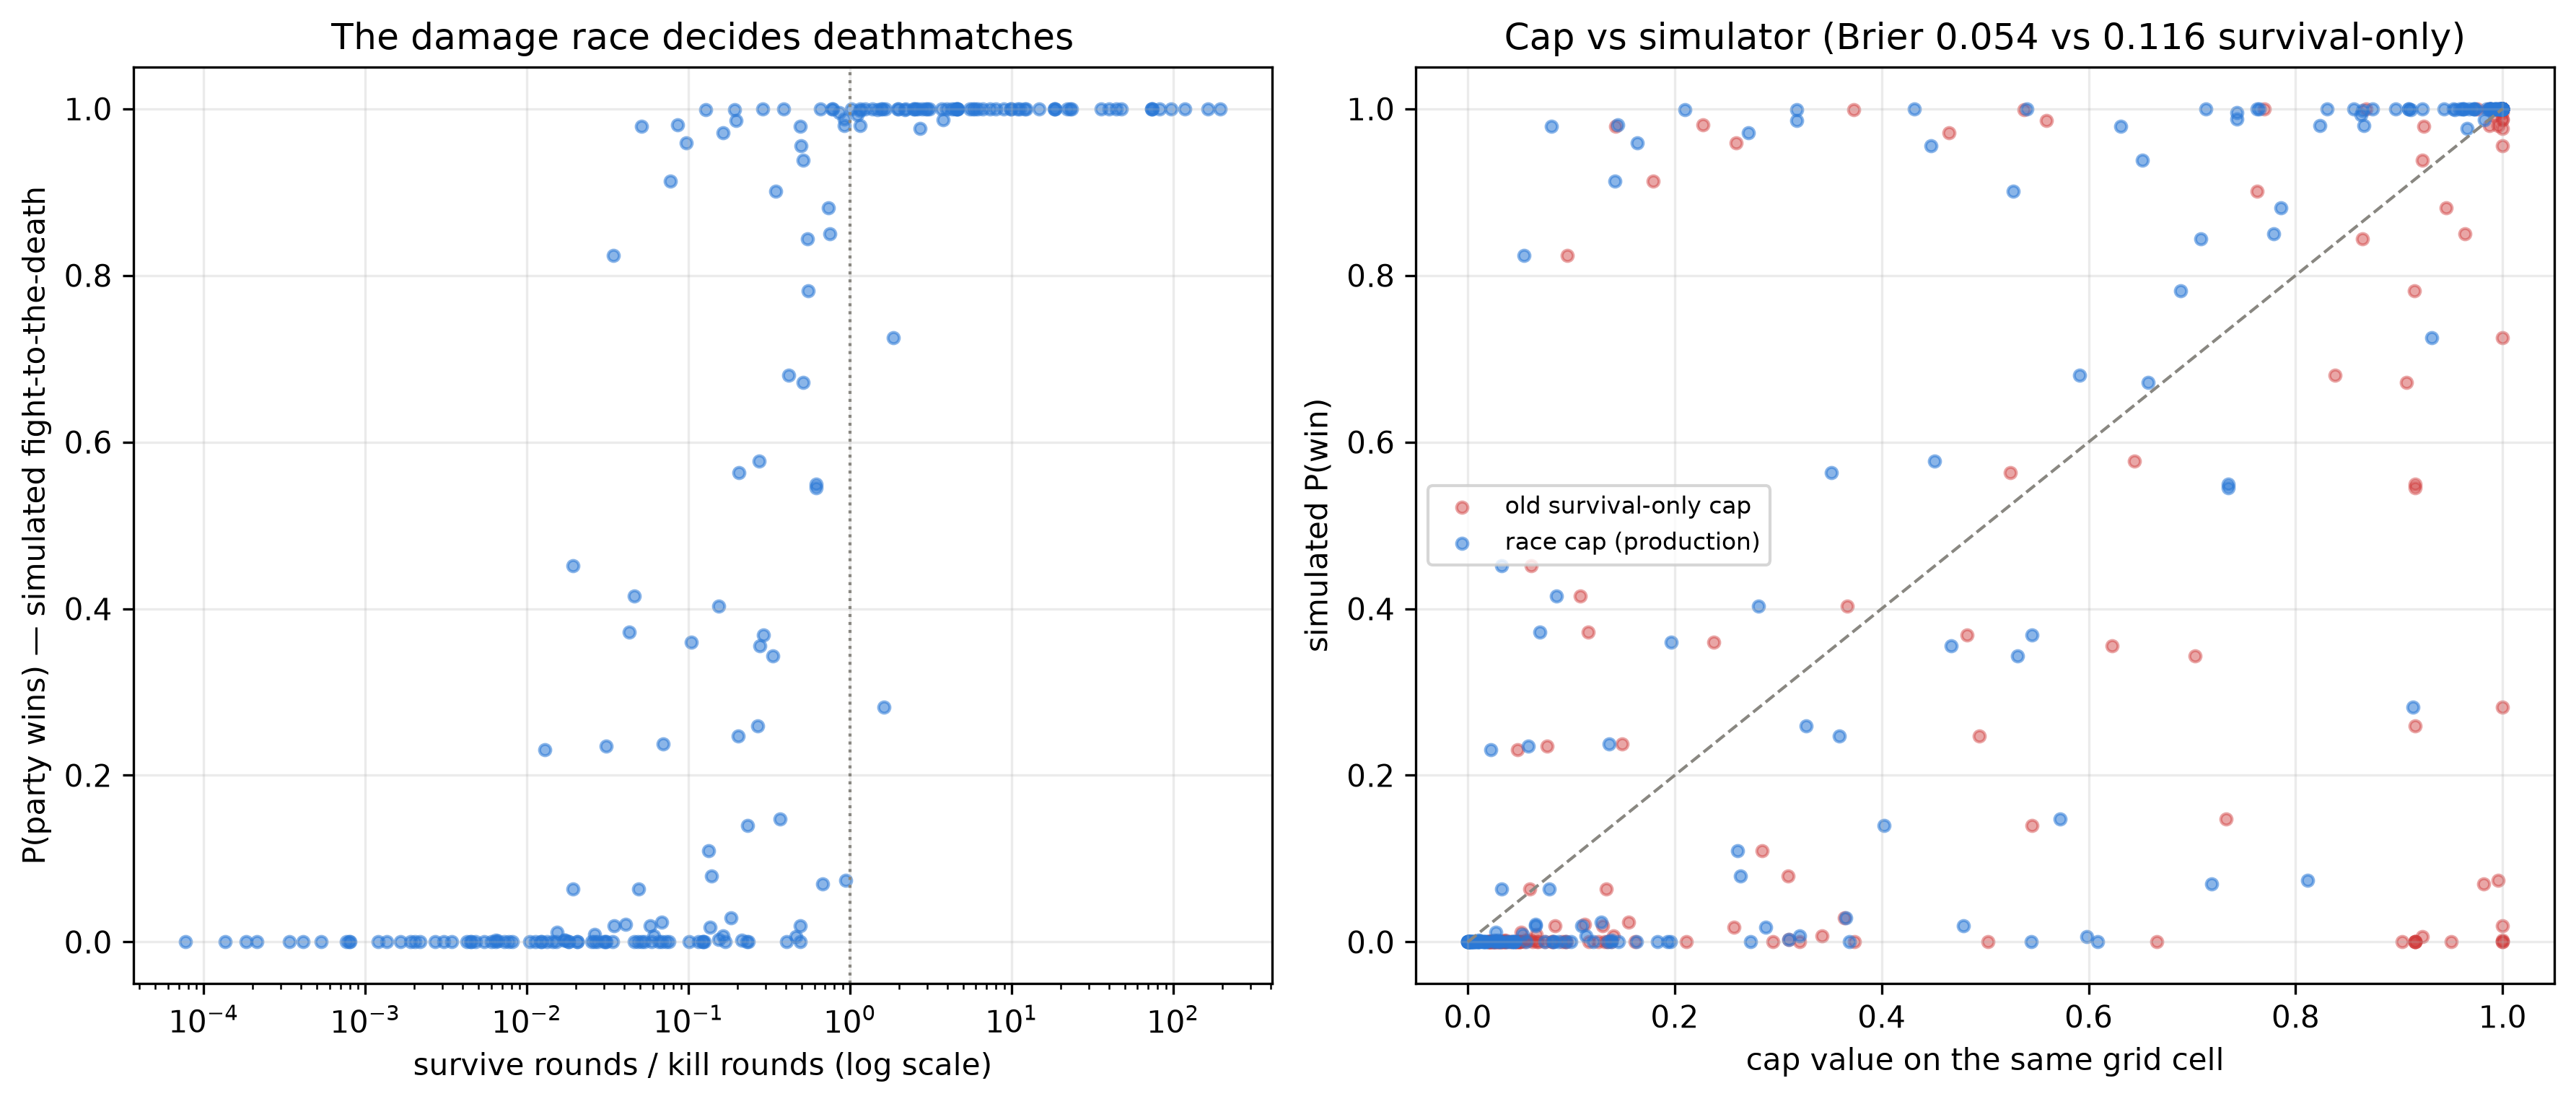
\includegraphics[width=\linewidth]{battlecast_guard_fit.png}
  \caption{Survival guard vs.\ deathmatch truth: 180 simulated cells, the calibrated
  fit (production) and the previous hand-tuned curve.}
  \label{fig:guard}
\end{figure}

\begin{figure}[t]
  \centering
  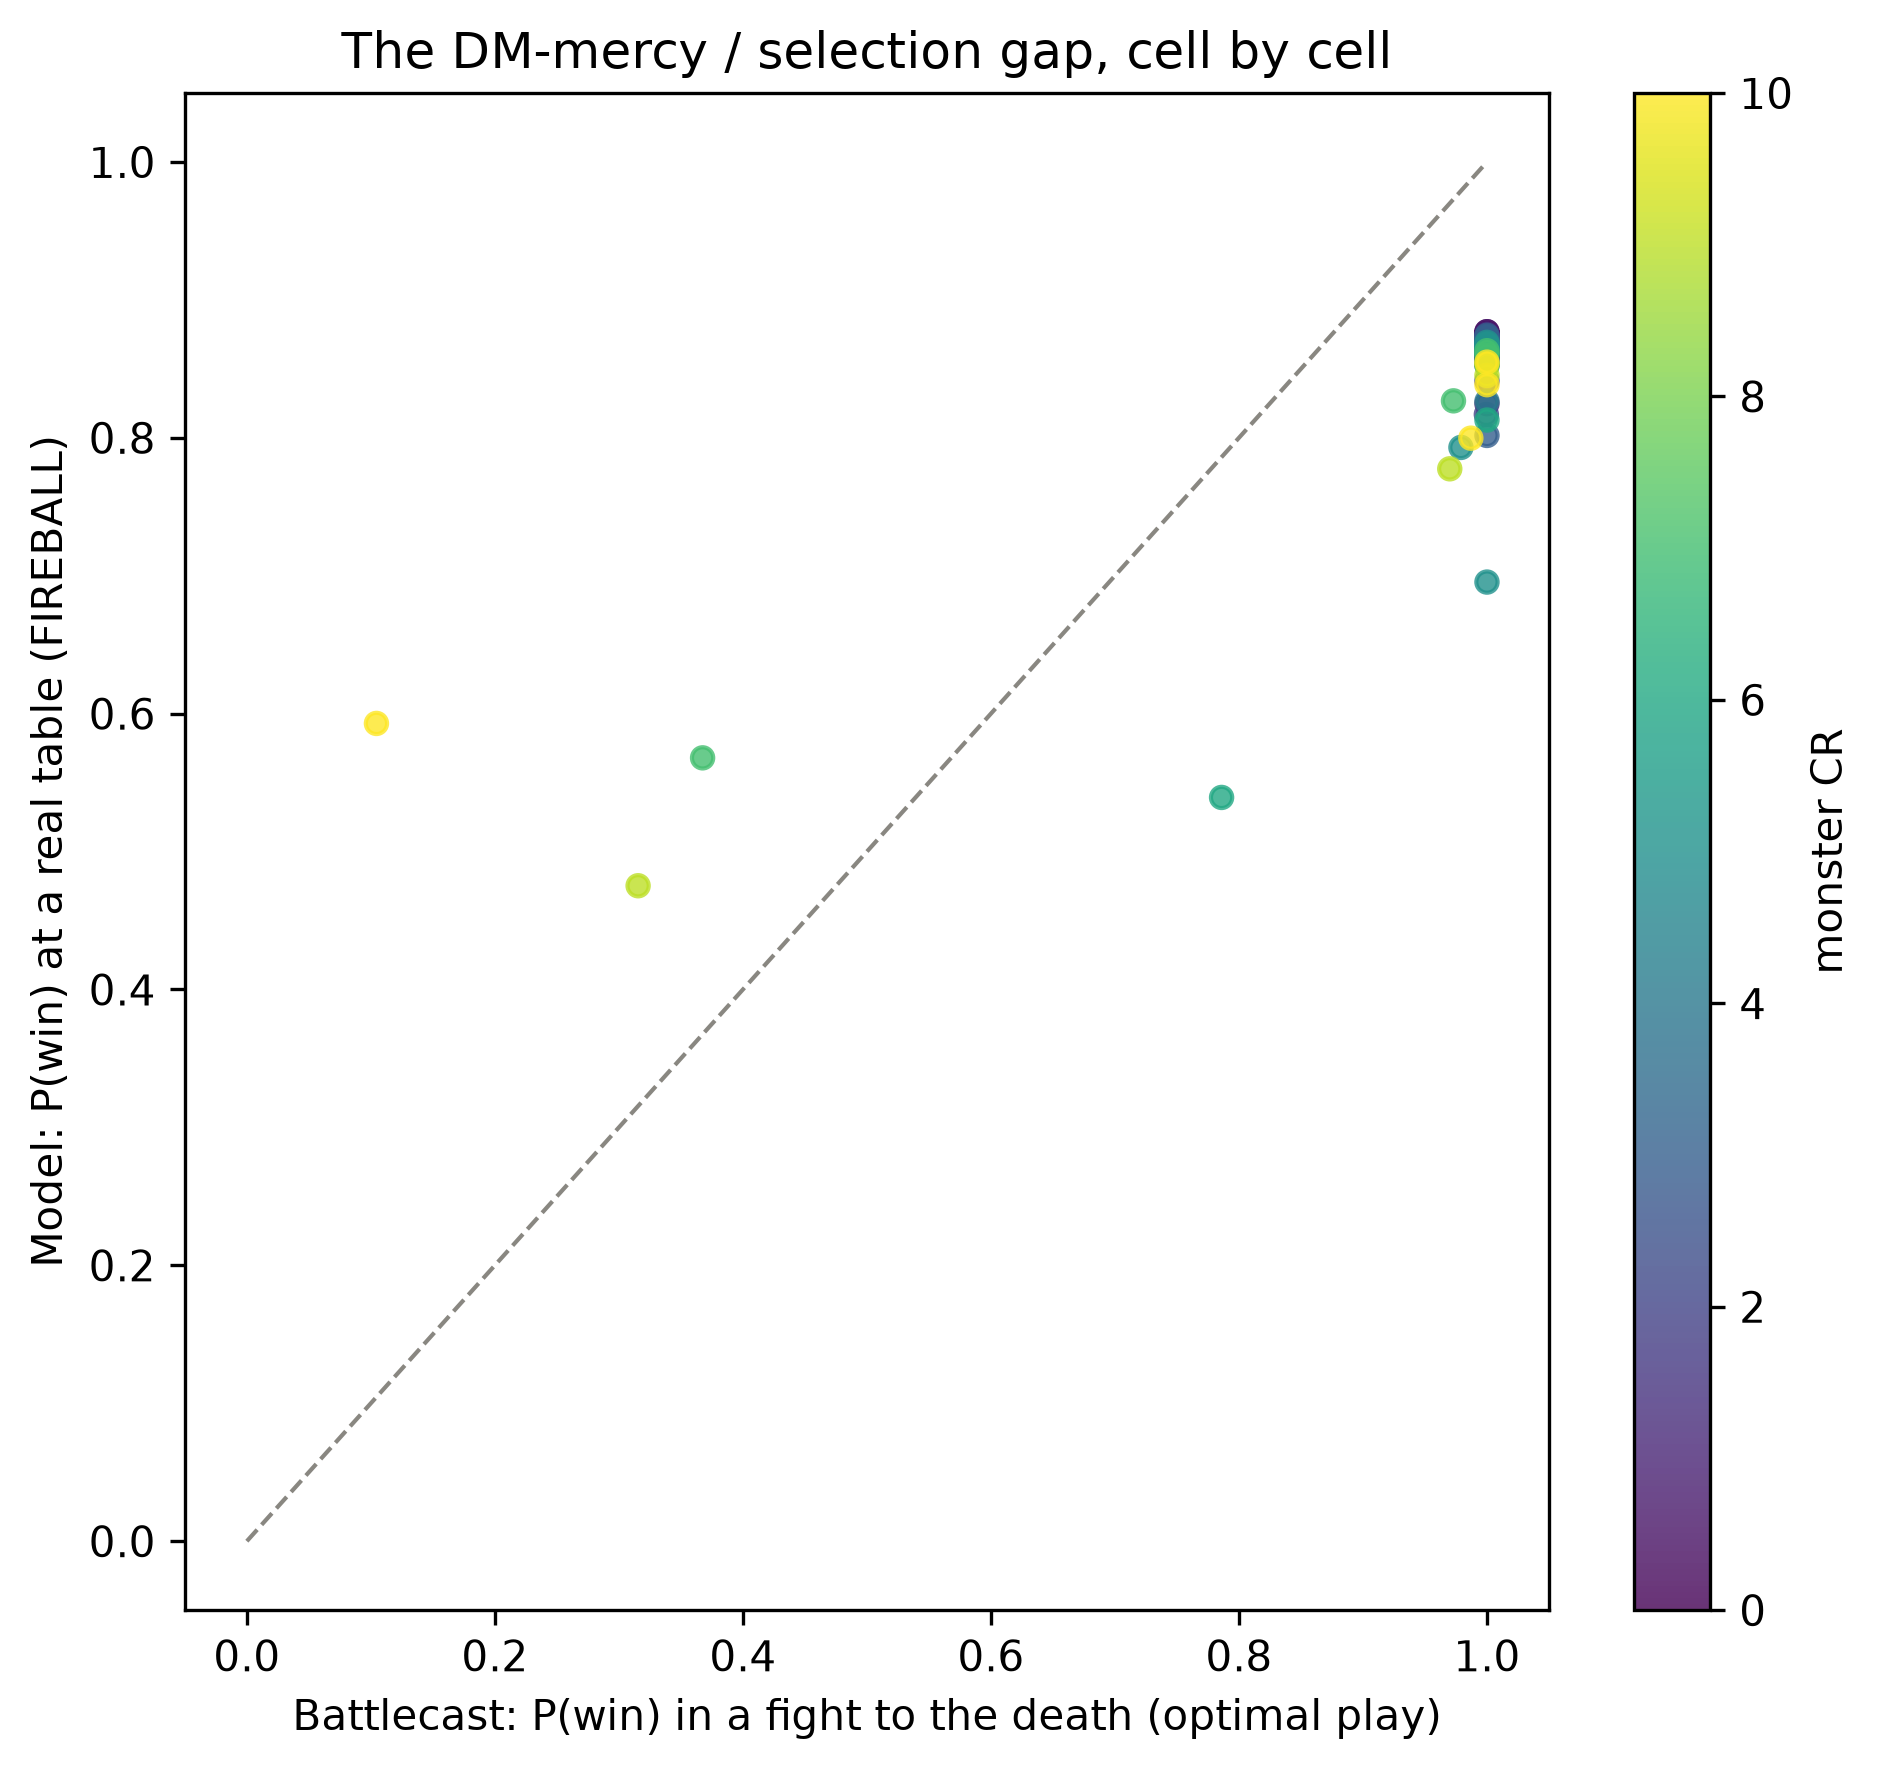
\includegraphics[width=\linewidth]{battlecast_mercy_gap.png}
  \caption{DM mercy quantified: model (table reality) vs.\ simulator (deathmatch),
  one point per encounter, color = CR.}
  \label{fig:mercy}
\end{figure}

\section{Results}
\subsection{Held-out performance}
Table~\ref{tab:main} reports performance on held-out campaigns. Calibration is
tight where the data mass lives (predicted 0.8--0.9), with mild overconfidence in
the lowest bins (Fig.~\ref{fig:calib}). Native TreeSHAP~\cite{shap} ranks party
level, monster size, nova pressure (\code{burst\_vs\_pc\_hp}), action economy
(\code{num\_monsters\_total}) and party hit chance as the leading signals --- the
parsed offensive statistics the official bestiary lacks are first-class drivers.

\begin{table}[t]
\centering\footnotesize\setlength{\tabcolsep}{4pt}
\begin{tabular}{lcc}
\toprule
Metric (held-out, $n{=}7{,}106$) & Value & 95\% CI\\
\midrule
ROC--AUC & 0.657 & [0.638, 0.674]\\
Brier score & 0.139 & [0.134, 0.145]\\
PR--AUC & 0.874 & ---\\
Log loss & 0.447 & ---\\
Grouped 4-fold CV AUC & \multicolumn{2}{c}{$0.601 \pm 0.040$}\\
Base rate $P(\text{win})$ & \multicolumn{2}{c}{0.830}\\
\bottomrule
\end{tabular}
\caption{Production model, campaign-grouped evaluation.}
\label{tab:main}
\end{table}

\begin{figure}[t]
  \centering
  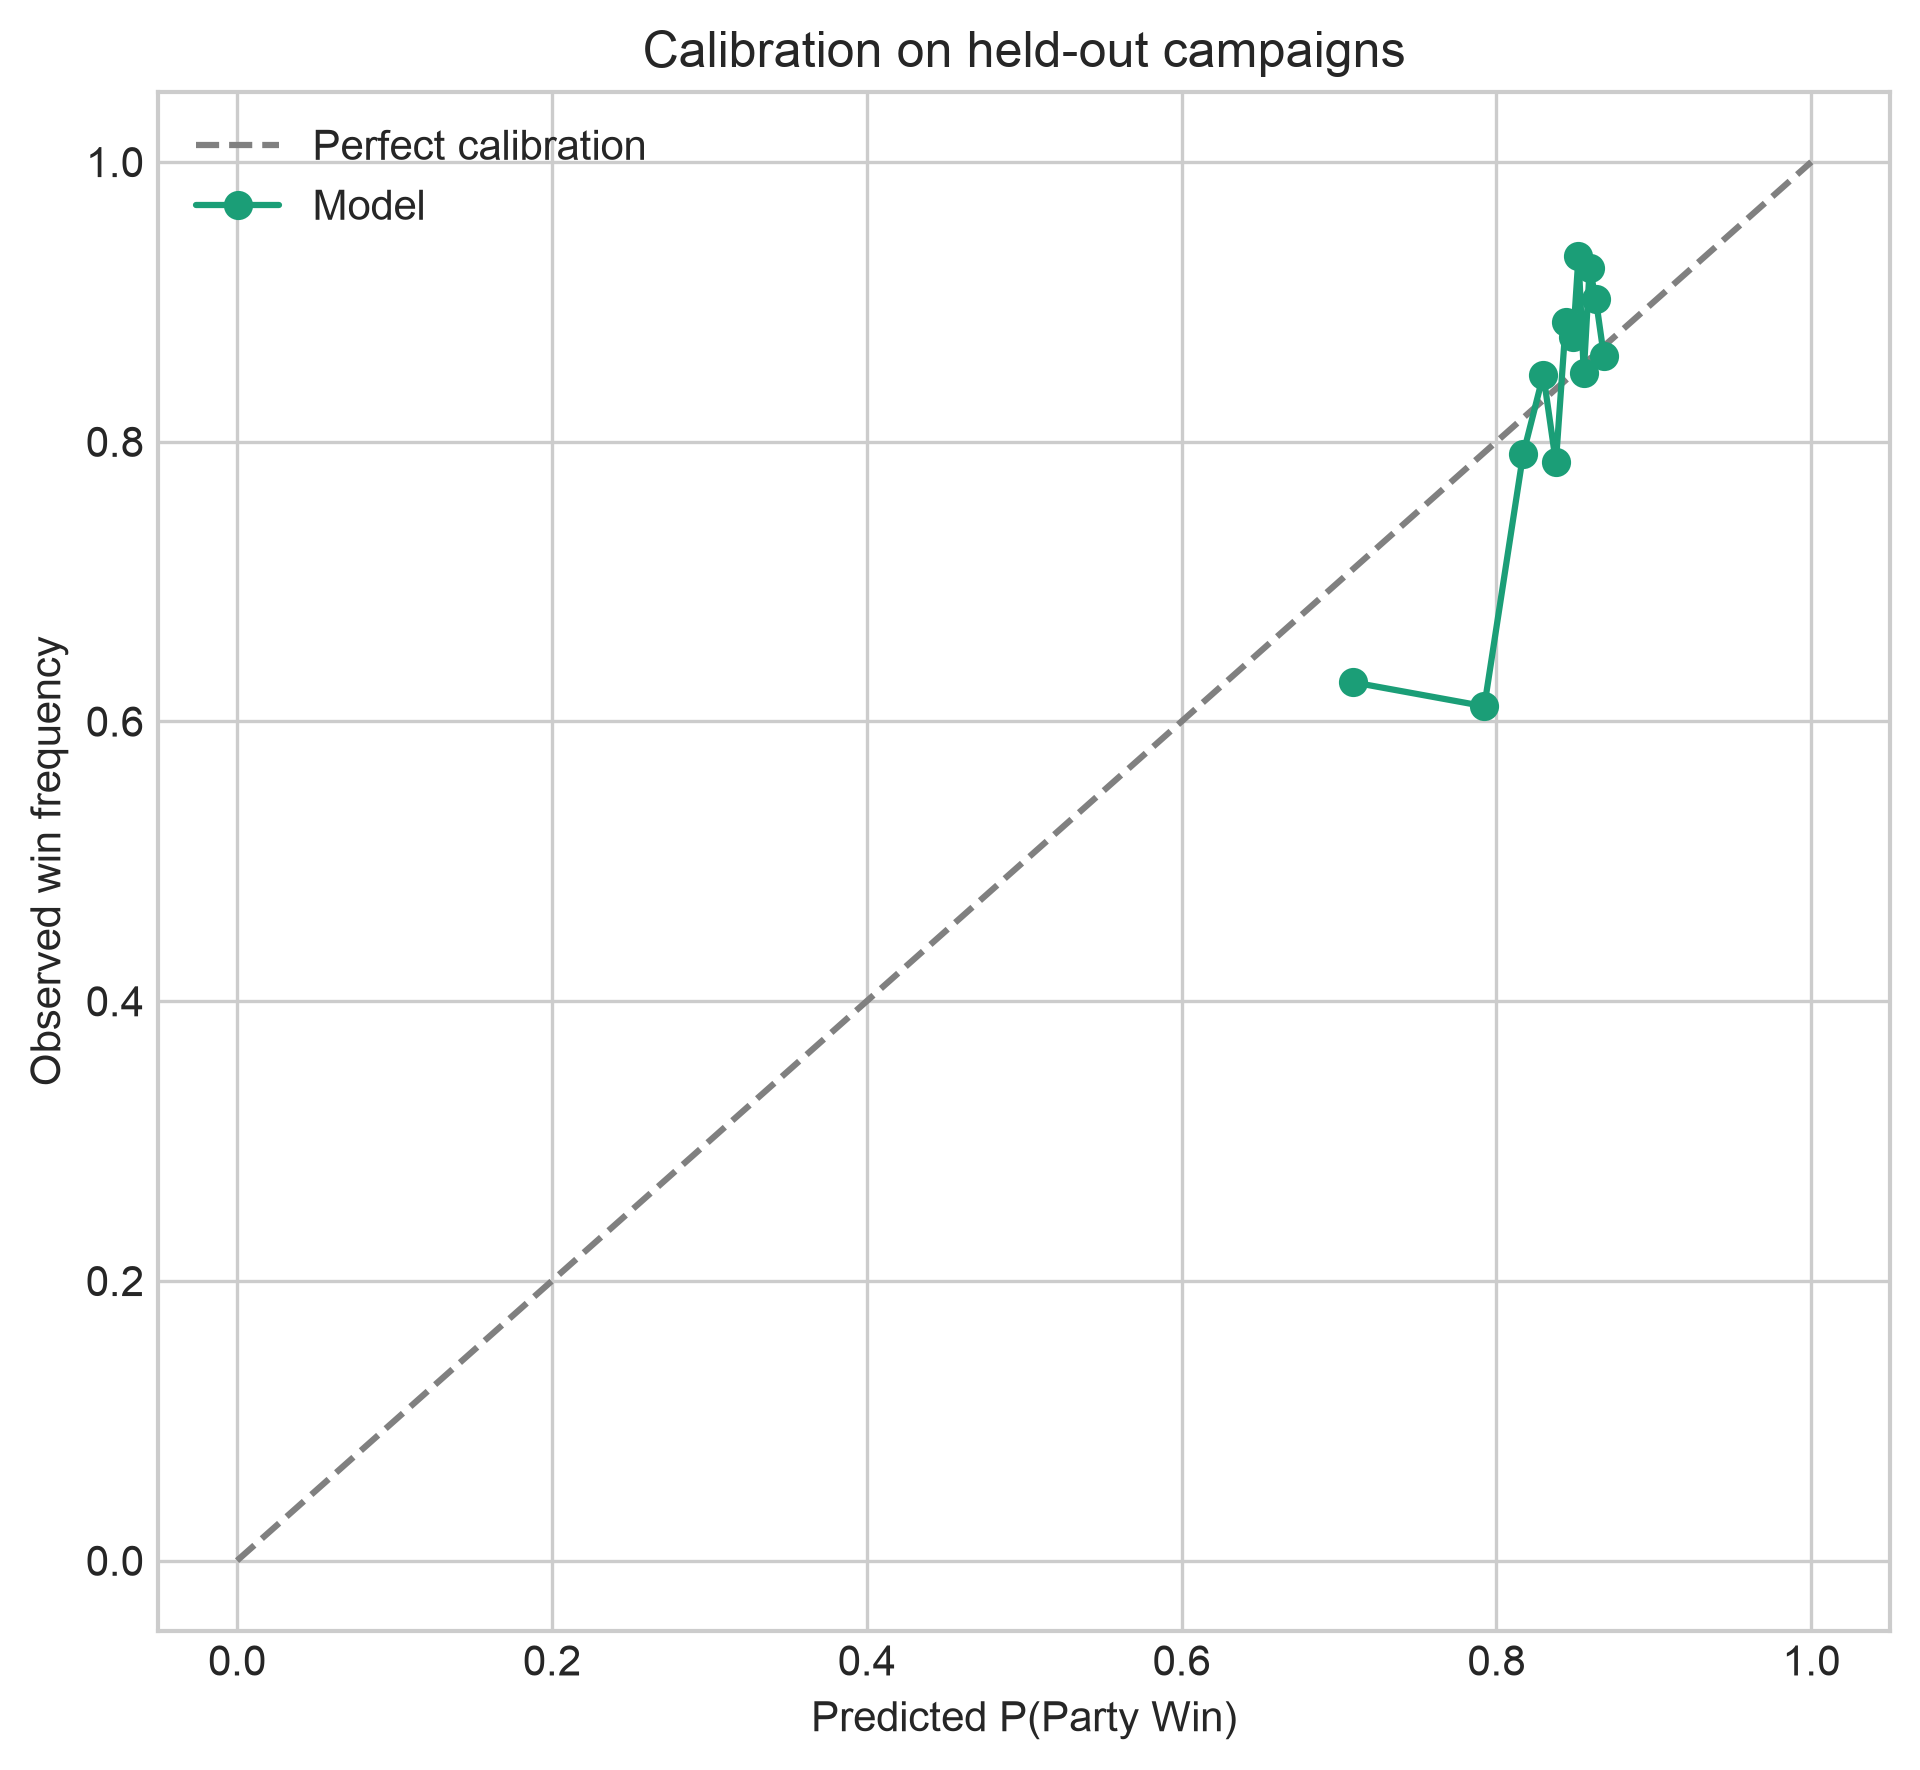
\includegraphics[width=.92\linewidth]{calibration_curve.png}
  \caption{Reliability on held-out campaigns.}
  \label{fig:calib}
\end{figure}

\subsection{Prediction $\neq$ decision}
Under identical grouped CV (Table~\ref{tab:zoo}), an $\ell_2$-penalized logistic
regression \emph{beats} the production model on observational risk. Promoted
experimentally to production, it rated 8 Liches as trivial and a 10{,}000-HP monster
as beatable: with no shape constraints, the linear fit absorbs selection confounding
--- its coefficients give \code{num\_monsters}, \code{total\_dpr} and \code{burst}
\emph{positive} signs and \code{avg\_party\_level} a \emph{negative} one (``stronger
parties lose more'', because stronger parties are served harder content). The
application's queries are interventional (``same monster, more of them''), so we
deploy the constrained model and accept ${\approx}0.04$ AUC as the price of
decision-grade behavior. The 13-axiom behavioral suite (count monotonicity, roster
dominance, level monotonicity, boundary verdicts, OOD flow) now gates every model
change.

\begin{table}[t]
\centering\footnotesize\setlength{\tabcolsep}{4pt}
\begin{tabular}{lcc}
\toprule
Model (identical grouped CV) & AUC $\pm$ sd & Brier\\
\midrule
Ridge logistic & $0.655 \pm 0.031$ & \textbf{0.136}\\
RFF kernel logistic~\cite{rff} & $0.624 \pm 0.013$ & 0.142\\
XGBoost + constraints (ours) & $0.614 \pm 0.033$ & 0.141\\
\bottomrule
\end{tabular}
\caption{Course model zoo. The linear model wins the metric and loses the job.}
\label{tab:zoo}
\end{table}

\subsection{Auxiliary analyses}
\textbf{Gaussian process.} On the 797-monster CR-prediction task, a GP
regressor~\cite{gpml} (RBF + white kernel, marginal-likelihood fitting) reaches MAE
0.86 vs.\ XGBoost's 0.94 ($R^2{=}0.954$) with 95\% predictive intervals achieving
\textbf{0.95 empirical coverage}.
\textbf{Synthetic balancing.} CTGAN~\cite{ctgan}-generated synthetic losses
(leakage-guarded: fitted on training campaigns only) used to ``balance'' the 83/17
classes degrade the same holdout to AUC 0.638 and Brier \textbf{0.186}, dragging the
predicted base rate to 0.61: with proper losses and calibration, imbalance was never
the problem, and resampling destroys calibration to fix it.

\section{The application}
A Streamlit appraiser (auto-deployed from \code{main}) exposes three modes ---
official bestiary (762 monsters with offense provenance badges), homebrew appraiser
(a CR predictor for ``what the book would print'', MAE 0.9, plus the True Lethality
Level), and a mixed-roster encounter builder aggregated exactly like training. Every
appraisal shows the by-the-book verdict next to the model's, win curves for five
party compositions, a party-size$\times$level heatmap, the fairest matchups with
official DMG tiers, and threat flags. The target win rate is a user-facing slider:
``fair'' is a policy, not a constant. Engineering: 61 unit tests + 13 behavioral
axioms (\code{make verify}), append-only experiment log, pinned environment,
one-command pipeline (\code{make retrain}).

\section{Limitations}
(i)~\emph{Observational ceiling}: dice variance, table tactics and unrecorded items
bound discrimination; AUC 0.657 with CIs is honest, not weak, at an 83\% base rate.
(ii)~\emph{Estimand mismatch} is handled by an explicit, sim-calibrated guard --- a
documented modeling choice, not end-to-end learning. (iii)~\emph{Simulator caveats}:
2024-SRD rules, optimized default builds, scripted play. (iv)~\emph{Thin support on
hard fights}: 96/100 mercy cells are deathmatch-easy; future work includes VTT
instrumentation, 30-second post-encounter forms with explicit retreat/fudge labels
(turning mercy into a censoring variable), and an all-SRD replay grid.

\section{Conclusions}
Five lessons travel beyond the game. Validate by the unit of leakage or every number
is fiction; calibrate when the product consumes probabilities, and measure it; a
better-AUC model can be unusable --- constraints encode the difference between
prediction and decision; know your estimand, because observational data cannot answer
counterfactual questions while simulation can (and can even calibrate your priors);
and the rulebook deserved a fair trial --- honestly implemented, it still loses to
34{,}907 real fights.

\begin{thebibliography}{9}\small
\bibitem{fireball} A.~Zhu et al. FIREBALL: A Dataset of Dungeons and Dragons
Actual-Play with Structured Game State Information. \emph{ACL}, 2023.
\bibitem{dmg} Wizards of the Coast. \emph{Dungeon Master's Guide}, pp.~82--83, 274. 2014.
\bibitem{xgboost} T.~Chen and C.~Guestrin. XGBoost: A Scalable Tree Boosting System.
\emph{KDD}, 2016.
\bibitem{optuna} T.~Akiba et al. Optuna: A Next-generation Hyperparameter
Optimization Framework. \emph{KDD}, 2019.
\bibitem{platt} J.~Platt. Probabilistic Outputs for Support Vector Machines.
\emph{Advances in Large Margin Classifiers}, 1999.
\bibitem{rff} A.~Rahimi and B.~Recht. Random Features for Large-Scale Kernel
Machines. \emph{NeurIPS}, 2007.
\bibitem{mmd} A.~Gretton et al. A Kernel Two-Sample Test. \emph{JMLR}, 13, 2012.
\bibitem{gpml} C.~E.~Rasmussen and C.~K.~I.~Williams. \emph{Gaussian Processes for
Machine Learning}. MIT Press, 2006.
\bibitem{ctgan} L.~Xu et al. Modeling Tabular Data using Conditional GAN.
\emph{NeurIPS}, 2019.
\bibitem{shap} S.~Lundberg and S.-I.~Lee. A Unified Approach to Interpreting Model
Predictions. \emph{NeurIPS}, 2017.
\end{thebibliography}

\end{document}
